

\documentclass{abstract_hutech}
\usepackage{color}
\usepackage{xcolor}
\usepackage{soul}
\usepackage[normalem]{ulem}


\newcommand{\REVIEW}[1]{\textcolor{blue}{#1}} % REVIEW is necessary later
\newcommand{\review}[1]{\textcolor{blue}{#1}} % REVIEW is necessary later
\newcommand{\FIXME}[1]{\textcolor{red}{#1}} % should be fixed later
\newcommand{\fixme}[1]{\textcolor{red}{#1}} % should be fixed later
\newcommand{\TODO}[1]{\textcolor{purple}{#1}} % TODO
\newcommand{\todo}[1]{\textcolor{purple}{#1}} % TODO
\newcommand{\eg}{\textit{e.g.,}}
\newcommand{\etal}{\textit{et al.}}
\newcommand{\ie}{\textit{i.e.,}}

\newcommand{\SJ}[1]{\textcolor{orange}{#1}} % for Sungjin
\newcommand{\CW}[1]{\textcolor{brown}{#1}} % for Chanwoo % using same color as Arvind (green hard to read..)
\newcommand{\AR}[1]{\textcolor{brown}{#1}} % for Arvind

\newcommand{\ours}{LSM-KVD}

\usepackage{hyperref}
\usepackage{subfig}
\begin{document}
\thispagestyle{firstpage}
\twocolumn[
	\begin{@twocolumnfalse}
	\vspace*{20pt}
	\begin{flushleft}
	\fontsize{20}{0}\selectfont{\textbf{~\ours{}: LSM-tree based Key-Value SSD}}
	\vspace{32pt}\par
	\fontsize{10}{12}\selectfont{\textbf{(Abstract) This is a template of Extended Abstract for HumanTech Paper Award. The recommended volume is 2 pages with 2-column format. Titles do not exceed two lines and abstracts do not exceed 15 lines.\\
		papers should be written in Times New Roman font with the font size of 20pt in bold for the title, 10pt in bold for abstracts, 11pt in bold for the titles within text, 10pt for the text, 9pt in bold for the titles of figures and tables and 9pt for the references. For the fairness of the review, Name, major, the school/university name, the school/university logo, and teacher/professors name of author should not be included in the abstract and paper.
	}}
\end{flushleft}
\vspace{20pt}
\end{@twocolumnfalse}
]

\section{INTRODUCTION}
\vspace{-5pt}
Key-Value store (KVS) has become a necessary infrastructure for many applications, such as caching, web indexing, and storage systems\iffalse cite{memcached,tao,bigtable,dynamo}\fi.  
Owing to its popularity and huge impact on application performance, serious efforts have been made to optimize KVS in various ways.  
Recently, offloading most of the key-value (KV) functionality onto a storage device has been suggested, the so-called KV-SSD\iffalse ~\cite{kvssd,kaml,nvmkv,bluecache}\fi.  
By making the storage hardware directly serve KV requests via a driver, KV-SSDs enable clients to bypass the deep software stack in the host.
For example, by performing most commonly used operations of KV databases, such as RocksDB\iffalse ~\cite{rocksdb}\fi, 
in KV-SSDs, we not only improve I/O latency and throughput of the operations but also reduce host resources ~\ie{CPU cycles, Memory}.

The existing ideas using hash algorithm for managing KV pairs because it has a simple architecture.
However, if the DRAM size is not large enough to hold all the hash entries, parts of the hash table must be stored in flash.
This inevitably involves expensive flash accesses to look for a key when it is not found in the DRAM-resident hash table.  
Even worse, if a hash collision occurs then multiple flash accesses may be required, resulting in long tail latency and drop in throughput.

%To confirm our analysis, we carried out experiments using a KV-SSD product (3.84~TB PM983~\cite{pm983,kv-pm983}).
%We were running workloads two phase, ~\texttt{load,run} with variable working set from 1GB to 3TB.
%In the load phase, there is only ~\texttt{SET} operation.
%After the first phase, we tested ~\texttt{GET} operation for 10 minutes. 
%Figure ~\ref{fig:hash-kvssd-exp} shows the results which performance is more degraded with larger working sets.
%the reason is that hash collision and flash look-ups for mapping information stored in NAND.

An alternative to hashing is a \emph{log-structured merge tree} (LSM-tree)~\cite{lsm-tree} which can be widely used for KV-store.
However, it has not only bad average read performance, 
but also additional overheads for the writing called compaction.
Since the compaction requires sorting keys which is a CPU-intensive job,
it can become a huge burden on embedded CPUs in SSD controllers. 
Also extra I/O operations to keep KV pairs sorted further deteriorate I/O throughput.  
Due to these drawbacks, LSM-tree has not been considered an attractive solution for KV-SSDs.

%\begin{figure}[t]
%%    \centering
%    \subfloat[IOPS of read]{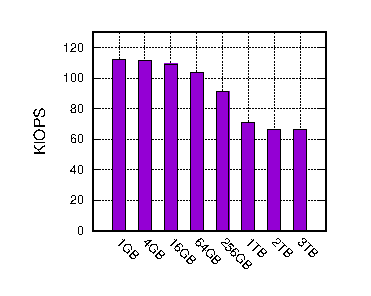
\includegraphics[width=0.24\textwidth]{exp/blkssd_throughput/throughput_compare.eps}}
%    \subfloat[CDF of read latency]{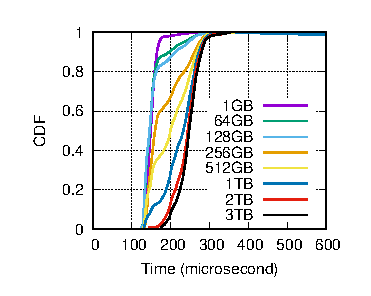
\includegraphics[width=0.23\textwidth]{exp/kvssd_latency_iops/kvssd_latency/kvssd_rlatency_trend.eps}}
%   %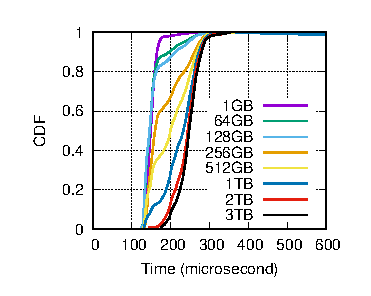
\includegraphics[width=0.24\textwidth]{exp/kvssd_latency_iops/kvssd_latency/kvssd_rlatency_trend.eps}
%    \caption{Experimental results with KV-SSD. Size of a key is 32B and Size of a value is 1KB.}\vspace{-13pt}
%    \label{fig:hash-kvssd-exp}
%\end{figure}
%
In this paper, by optimizing the LSM-tree algorithm and tightly integrating it with an SSD controller, LSM-tree-based KV-SSDs can outperform hash-based designs.  
Our solution is based on three ideas.
First, pin all KV indices of the top levels of the tree to DRAM to speedup reads.
This level pinning not only guarantees the worst-case read latency, but improves average latency by reducing flash look-ups for retrieving KV indices.  
Second, run sorting tasks using HW accelerators, in parallel with I/O tasks to eliminate CPU overheads for compaction.
Third, combine level-pinning with key-value separation~\cite{wisckey} to reduce I/O overheads for compaction.
Collectively these techniques remove the compaction bottleneck and provide high write-throughput.

Additionally, due to the first idea, we can extend the design space of LSM-tree-based KV-SSD by using trade-off between DRAM requirements and the performance.
We believe that our techniques can also be applied profitably to general LSM-tree implementations, which may not have the same resource constraints as KV-SSDs do.

%Based on these ideas, we have designed a new LSM-tree-based KV-SSD, called
%\textit{\ours{}} and implemented it on an FPGA-based SSD
%platform~\cite{bluedbm}. 
%It is well known that the LSM-tree offers an intrinsic tradeoff between
%read-latency and write-throughput. We have quantified this tradeoff and shown that for
%a given DRAM capacity an application can configure our implementation to
%support its KV performance requirements.
\vspace{-10pt}
\section{\ours{}}\vspace{-20pt}
\begin{figure}[h]
	\centering
	%\subfloat[layout]{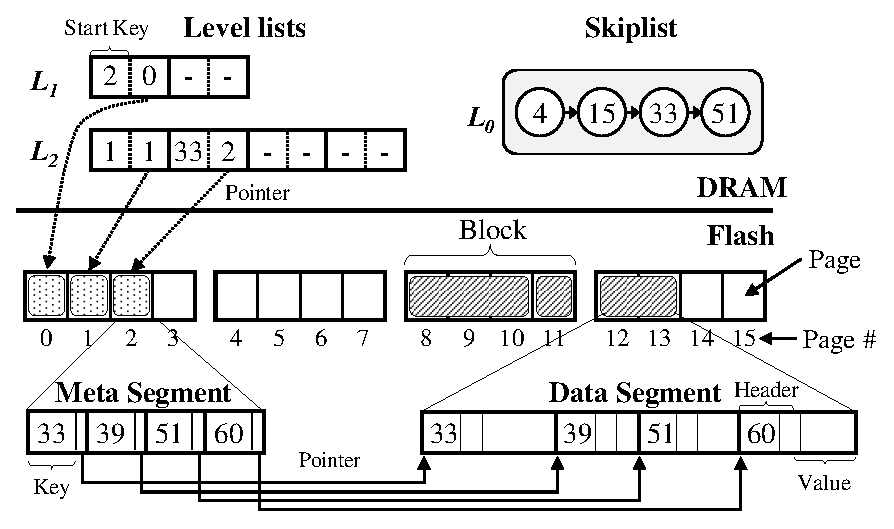
\includegraphics[width=0.24\textwidth]{fig/fig3.eps}}
	%\subfloat[Flush & Compaction]{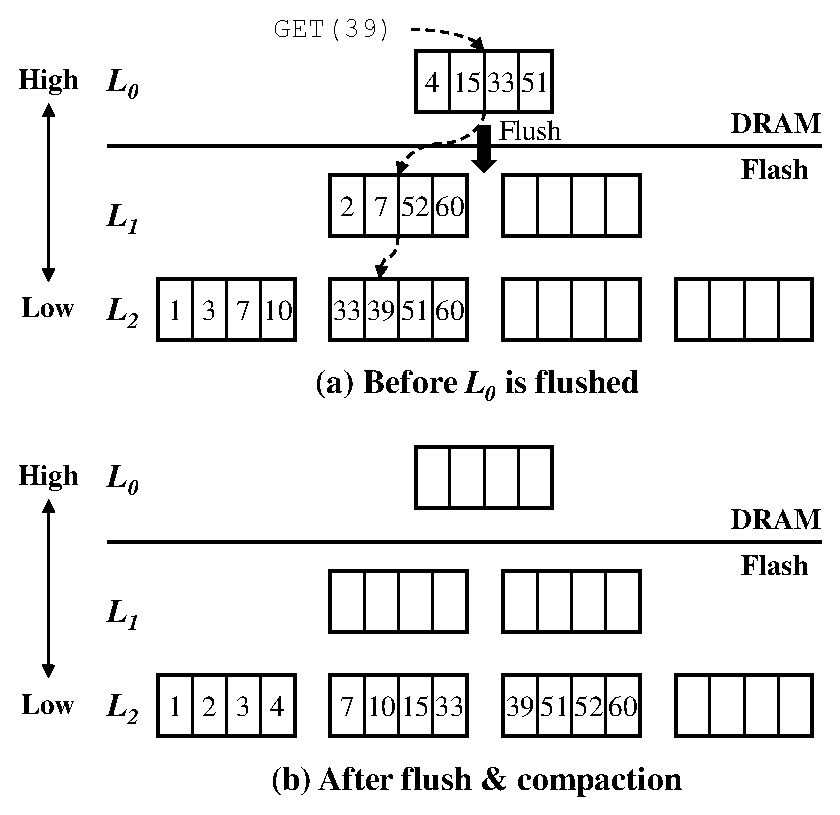
\includegraphics[width=0.24\textwidth]{fig/fig1.eps}}
	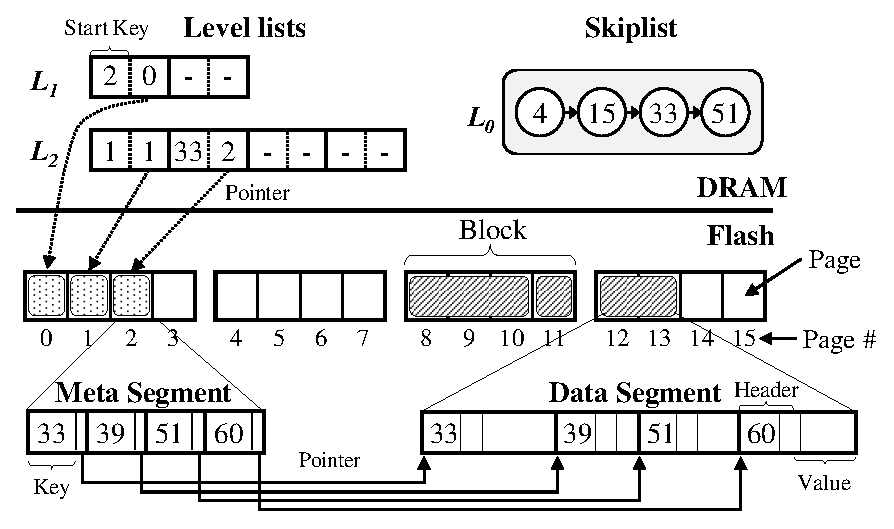
\includegraphics[height=4.0cm]{fig/fig3.eps}
	\caption{LSMKVD Layout}
	\label{fig:overall}\vspace{-20pt}
\end{figure}
\subsection{Design of \ours{}}\vspace{-5pt}
\ours{} has four types of data structures to implement the LSM-tree algorithm
(Figure~\ref{fig:overall}): a \textit{skiplist} and \textit{level lists}, which
all reside in DRAM, and  \textit{meta segments} and \textit{data segments},
which all reside in flash. The skiplist corresponds to $L_0$ in the LSM-tree algorithm, and holds KV
objects as large as enough to fully utilize the parallelism of a NAND chip
array.  Each skiplist entry has four fields: <key size, key, value size,
value>, and the skiplist is kept sorted by the keys. 
When the skiplist is full, it flush all KV pairs in skiplist into data segments and make a new meta segment for the flushed KV objects.
The new meta segment is also written into the flash, and inserted into $L_1$ \textit{level list}.

\textit{level list} keeps track of meta segments at every level in the flash, Each level list is an array of pointers(4B each)
to meta segments belonging to the level. 
Each array entry also contains the start key (a variable size from 16B to 128B) of the meta segment to facilitate searching.
Figure~\ref{fig:overall} illustrates examples of how the level lists point to 
meta segments which, in turn, point to actual values.
when a specific level({$L_n$}) list is full, the level list compacts with below level({$L_{n+1}$}) list and becomes a new lower level({$L_{n+1}$}).
%In our design, each meta segment belongs to one of the levels in the tree.
%\ours{} maintains another in-memory data structure, \textit{level lists}, which
%keeps track of meta segments at every level in the flash.  Each level list is
%an array of pointers (4 B each) to meta segments belonging to the level.  Each array
%entry also contains the start key (a variable size from 16 B to 128 B) of the meta segment to facilitate searching.
%Figure~\ref{fig:overall} illustrates examples of how the level lists point to
%meta segments which, in turn, point to actual values.

\vspace{-5pt}
\subsection{DRAM Requirements Comparison}\vspace{-5pt}
Let's estimate DRAM requirements of~\ours{} and Hash-based KV-SSD.
We assume that an SSD capacity is 4 TB and each meta segment is 32 KB.
First consider the case where the average sizes of keys and values are 32 B and 1 KB,
respectively~\cite{kvsize}. In this case only 162 MB DRAM is needed to hold all the level lists.
For the worst-case scenario, where all the objects have the maximum key size of 128 B,
the level lists would require about 2.1 GB DRAM. 
This can still easily fit in 4 GB DRAM that 4 TB SSD has for mapping.

However, in case of Hash-based one, it needed at least 144GB DRAM in 32B keys and 1KB values setting.
To reduce DRAM size, some use signature instead of key ~\cite{bluedbm} by hashing its key.
Although it reduces the DRAM requirements to 24GB which is calculated when its each signature size is 2B, it is too huge to fit caching all the mapping.
It means that even using the signature design it should store some part of the mapping in flash chips.
And it also occur another type of collision ~\ie{the different two keys can have a same signature}.


\vspace{-5pt}
\subsection{Optimizing Technics}\vspace{-5pt}
\textbf{Optimizing Read Latency:}
The traditional LSM-tree uses bloom filter for optimizing read. 
But ~\ours{} adopts more aggressive strategy: \textit{level pinning}. 
If the LSM-tree has $n$ levels, \ours{} keeps meta segments for top-$k$ levels ($k \le n-1$) in DRAM.
To process a \texttt{GET} request, it first searches for a key in top-$k$
levels in DRAM.  Only when a key is not found there, it lookups the rest
of levels resident in the flash.
%With the level pinning, the number of the worst-case flash lookups is reduced to $O(n-k-1)$. 

\textbf{Optimizing Compaction:}
To keep each level sorted, \ours{} performs compaction which involves extra I/Os and CPU cycles.
By using \textit{level pinning} and seperating keys from values{~\cite{wisckey}}, it can reduce I/O traffics in compaction phase. 
However, The sorting overhead of compaction is pretty huge on embedded system. 
We address this problem by offloading sorting tasks to a special hardware accelerator in the SSD controller.

\vspace{-5pt}
\subsection{Memory and Performance Trade-offs}\vspace{-5pt}
Thanks to \textit{level pinning}, We extend LSM-tree design trade-off using not only the height but also number of pinned levels. 
The original cost formation of LSM-tree's average write throughput and worst look-up cost are 
$O((n-1)\cdot\frac{R^{1/(n-1)}}{B})$ and $O(n-1)$ 
where $R$ is the number of meta segments in as SSD, and $B$ is the average number of keys in a meta segment.

But when using \textit{level pinning}, 
the write costs and look-up costs are change to $O((n-k-1)\cdot\frac{R^{1/(n-1)}}{B})$ and $O(n-k-1)$ respectively.
Also the DRAM requirements of \textit{level pinning} can be modeled $\sum_{i=1}^{k}(R^{1/(n-1)})^i\cdot M$ where $M$ is the size of a meta segment.
Thus, by using two parameters, We can more easily design ~\ours{} to fit DRAM size and performance requirements.

\vspace{-5pt}
\section{EXPERIMENTS}\vspace{-5pt}
\subsection{Experimental Setup}\vspace{-5pt}
We implemented the \ours{} software and hardware accelerator on our FPGA-based
SSD platform that has a quad-core ARM Cortex-A53 CPU running at 1.2 GHz with 16 GB
DRAM. This hardware specification is almost equivalent to those of recent SSDs.
And we scaled down the SSDs capacity to 64GB which is originally 256GB. Available DRAM for KV indexing was set to 64MB.

For realistic experiments, We implemented the hash-based KVSSD using 8-bit signature,
which is sufficient to cache entries.
And \ours{} is pinning top 3 levels among the total 5 levels.
To confirm effect of the HW-accelerator, We tested two diffrent versions of \ours.
One is \texttt{LSM-KVD}, another is \texttt{LSM-KVD+} which adopt the HW-accelerator
.
\begin{figure}[t]
	\centering
	\subfloat[IOPS]{\includegraphics[height=8cm,angle=-90]{./exp/exp1/exp1.eps}}\vspace{-13pt}
	\subfloat[CDF of read latency]{\includegraphics[height=8cm,angle=-90]{./exp/exp2/exp2.eps}}\vspace{2pt}
	\caption{
	\TODO{YCSB results of Hash-based KV-SSD and \ours{}}
	}
	\label{fig:result}
	\vspace{-17pt}
\end{figure}

\vspace{-10pt}
\subsection{YCSB}\vspace{-5pt}
We measured IOPS and read latency of the hash-based KV-SSDs and \ours{} while running YCSB with 32B keys and 1KB values setting.
YCSB has variable workloads on read,write ratio and workload pattern. Please see~\cite{YCSB} for workloads details.
%\todo{explanation of A,C,D,E workloads}.


\textbf{IOPS:}
Figure~\ref{fig:result} (a) shows IOPS result of YCSB.
\ours{} outperformed the
hash-based ones, providing 47\% higher IOPS, on average.
And thanks to the HW-accelerator, \texttt{LSM-KVD+} has better performance than \texttt{LSM-KVD} on all workloads including \texttt{SET} operation.

% Particularly, for
%YCSB-E with range queries, \ours{} showed 71$\sim$111\% higher IOPS thanks to
%LSM-tree's sorted nature. 
%In case of YCSB-C, Because \ours{} doesn't have any cache mechanism, It is weak when the workload has read after read the same key. 
%But In case of YCSB-D, otherwise, it performed very well because the workload's pattern is read after write same key. Almost keys were hitted in level pinning.
%

\textbf{Read Latency:}
Figure~\ref{fig:result} (b) shows CDF graphs of read response times of all three types of KVSSD from 95\% to 99.99\%.
\texttt{Hash} was suffer collision on all workloads. 
However, By using level pinning \ours{} can guarantee that \texttt{GET} can be done in two flash lookups.
Thus, \ours{} beat \texttt{Hash} on all workloads.
\vspace{-5pt}
\bibliographystyle{acm}
\bibliography{references.bib}
\end{document}
